% arara: pdflatex
% !arara: biber
% !arara: pdflatex
% How to run: 
% 1) pdflatex "filename".tex
% 2) biber "filename"
% 3) pdflatex "filename".tex
% 4) pdflatex "filename".tex


\documentclass[x11names]{article}
\usepackage{verbatim}
\usepackage{listings}
\usepackage{graphicx}
\usepackage{color}
\usepackage{amsmath}
\usepackage{amssymb}
\usepackage[T1]{fontenc}
\usepackage{shadow}
\usepackage{hyperref}
\usepackage{physics}
\usepackage{url}
%For use in pictures
\usepackage{tikz}
\usepackage{tikz-3dplot}
\usepackage{wrapfig}

\usepackage[l2tabu]{nag} %NAgs when using bad practices


\usepackage{subcaption}
\usepackage[utf8]{inputenc}
\usepackage{booktabs} % Allows the use of \toprule, \midrule and \bottomrule in tables
\usepackage[font={small,it}]{caption}
\usepackage[margin=0.7in]{geometry} %Sets the margins in the document
\usepackage{siunitx}    %Allows use of SI units macros

%Defines calculator way to write powers of ten
\sisetup{output-exponent-marker=\textsc{e}}


% Change numbering and some commands
\renewcommand\thesection{Exercise \Roman{section}}
\renewcommand\thesubsection{\Roman{section}.\alph{subsection}}

%% references
\usepackage[style=authoryear,
            bibstyle=authoryear,
            backend=biber,
            % refsection=chapter,
            maxbibnames=99,
            maxnames=2,
            firstinits=true,
            uniquename=init,
            natbib=true,
            dashed=false]{biblatex}

\addbibresource{bibliography.bib}

\usepackage[capitalize]{cleveref}

\setcounter{tocdepth}{2}

\lstset{language=c++}
\lstset{alsolanguage=[90]Fortran}
\lstset{basicstyle=\small}
\lstset{backgroundcolor=\color{white}}
\lstset{frame=single}
\lstset{stringstyle=\ttfamily}
\lstset{keywordstyle=\color{red}\bfseries}
\lstset{commentstyle=\itshape\color{blue}}
\lstset{showspaces=false}
\lstset{showstringspaces=false}
\lstset{showtabs=false}
\lstset{breaklines}


\definecolor{keywords}{RGB}{255,0,90}
      \definecolor{comments}{RGB}{0,0,113}
      \definecolor{red}{RGB}{160,0,0}
      \definecolor{green}{RGB}{0,150,0}
       
      \lstset{language=Python, 
              basicstyle=\ttfamily\small, 
              keywordstyle=\color{keywords},
              commentstyle=\color{comments},
              stringstyle=\color{red},
              showstringspaces=false,
              identifierstyle=\color{green}
              }



\title{ Exercise 9 \\ Sommerjobb Numeriske Plasmaoppgaver }
\author{Gullik Vetvik Killie
		}

\renewcommand{\va}{\vec}

%%%%%%%%%%%%%%%%%%%%%%%%%%%%%%%%%%%%%%%%%%%%%%%%%%%%%%%%%%%%%%%%%%%%%%%%%%%%%%%%%%%%
% Actual text starts here
%%%%%%%%%%%%%%%%%%%%%%%%%%%%%%%%%%%%%%%%%%%%%%%%%%%%%%%%%%%%%%%%%%%%%%%%%%%%%%%%%%%%
\begin{document}


\maketitle

\section{}

\subsection{Theory}
  In this exercise we will investigate how electrically charged particles behave in the converging magnetic field above the north pole and the balance between the forces.
\\ \\
  A particle gyrating in will have a magnetic moment, dependant on it's perpendicular velocity, given by

  \begin{align}
    \va{\mu} &= \frac{mv_\perp^2}{2B} \va{e}_B
  \end{align}

  The gradient force felt by the particle is then given by

  \begin{align}
    \va{F}_B &= -\left( \va{\mu}\cdot\nabla \right)\va{B}
  \end{align}

  The particle will also feel a gravitational force and the force balance is given when these 2 forces are equal.

  \begin{align}
    -\va{F}_G + \va{F}_B &= 0  
    \\
    mg(z) &= \frac{mv_\perp^2}{2B(z)} \pdv{B_z(z)}{z}
  \end{align}
  \noindent If we let the magnetic field be approximated as in the previous exercises,

  \begin{align}
    \va{B}(\va{r}) &= \frac{\mu_0}{4\pi}\left( \frac{3\va{r}(\va{r}\cdot\va{m}  )}{r^5} - \frac{\va{m}}{r^3} \right)
    \\
    \va{g}(\va{r}) &= - \gamma \frac{M_e}{r^3}
      \begin{pmatrix}
        x \\ y \\ z
      \end{pmatrix}
  \end{align}

  \noindent if we then consider the case where the guiding center of the particle is \(200 \si{\kilo\meter}\) straight above the magnetic north, so the guiding center coordinates is
  \( \va{r}_0 = (0,0,200\si{\kilo\meter} + R_e)\). Then it becomes simpler to find the z directed part of the gradient.

  \begin{align}
    \pdv{B_z(z)}{z} &= \pdv{}{z}\left( \frac{\mu_0}{4\pi} \left(\frac{3z^2m_z}{z^5} - \frac{m_z}{z^3} \right)\right)
    \\
    &= \frac{\mu_0m_z}{4\pi} \left( - \frac{9}{z^4} + \frac{3}{z^4} \right)
    \\
    &= - \frac{3\mu_0m_z}{2\pi z^4}
  \end{align}

  Then the gyration velocity giving a balance in the force given by:

  \begin{align}
    v^2_\perp &=  2B(z)g(z) \left(\pdv{B_z(z)}{z} \right)^{-1}
  \end{align}
  Assuming that the particle is directly above the magnetic north pole, so the radius is given by the \(z\)-coordinate, the 3 factors become:
   \begin{align}
    \begin{split}
      B(z) &= \frac{\mu_0}{4\pi}\left( \frac{3z^2m_z}{z^5} - \frac{m_z}{z^3} \right) =  \frac{\mu_0 m_z}{2\pi z^3} \approx \frac{4\pi \times 10^{-7} \times 7.94 \times 10^{22}}{2\pi\times (6.571\times 10^6 \si{m})^3} \si{\tesla}\approx 5.597\times 10 ^{-5} \si{\tesla}
      \\
      g(z) &= - \gamma \frac{M_e}{z^3} z = -\frac{\gamma M_e}{z^2} \approx - \frac{6.7 \times 10^{-11} \times 5.9 \times 10^{24}}{(6.571\times 10^6 )^2} \si{\meter \per \second^2} \approx -9.1 \si{\meter\per\second^2}
      \\
      \pdv{B_z(z)}{z} &= - \frac{3\mu_0m_z}{2\pi z^4} \approx -\frac{6 \times 10^{-7}\times 7.94\times 10^{22}}{(6.571\times 10^6 )^4 } \si{\tesla \per\meter } \approx -2.55\times 10^{-11} \si{\tesla \per\meter }
    \end{split}
    \intertext{and the total initial perpendicular velocity will be}
    v_\perp &\approx \sqrt{ (5.597\times 10 ^{-5} \si{\tesla}) \times (-9.1 \si{\meter\per\second^2}) / (2.55\times 10^{-11} \si{\tesla \per\meter } )} \approx 6300 \si{\meter\per\second}
  \end{align}
  

\subsection{Results}

  \begin{figure}
      \centering
      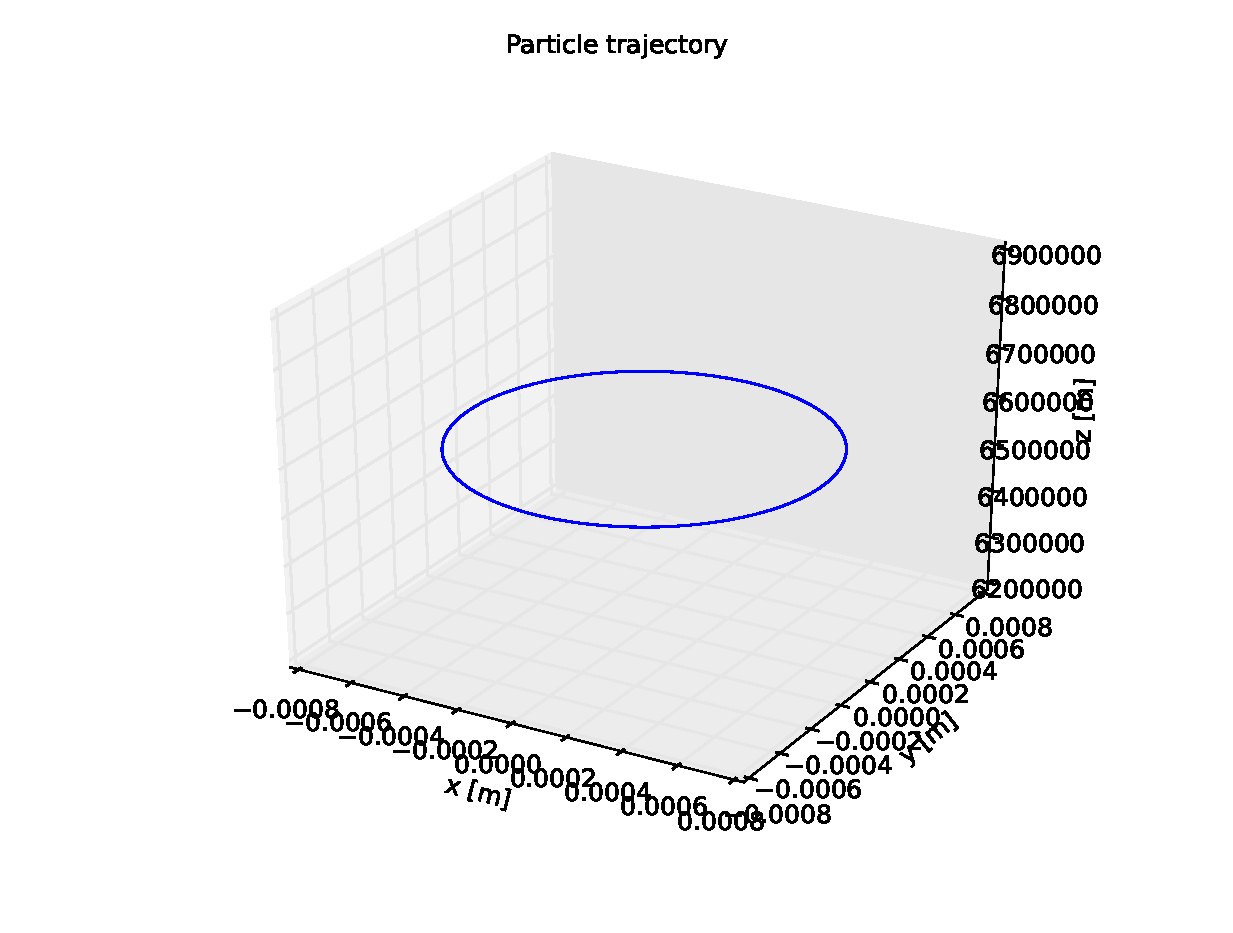
\includegraphics[width = 0.30\textwidth]{figures/7_0_12_3Dplot}
      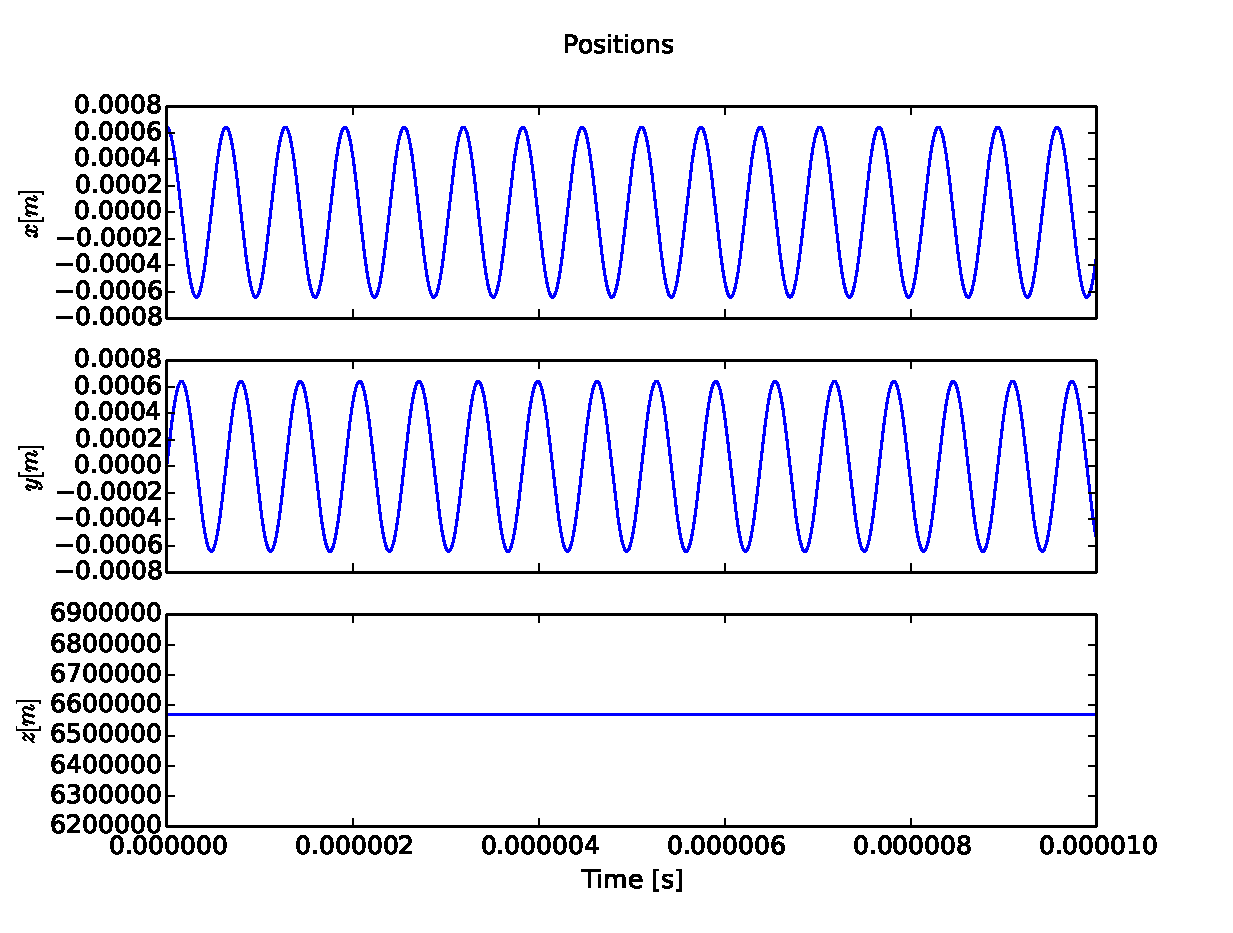
\includegraphics[width = 0.30\textwidth]{figures/7_0_12_xyz}
      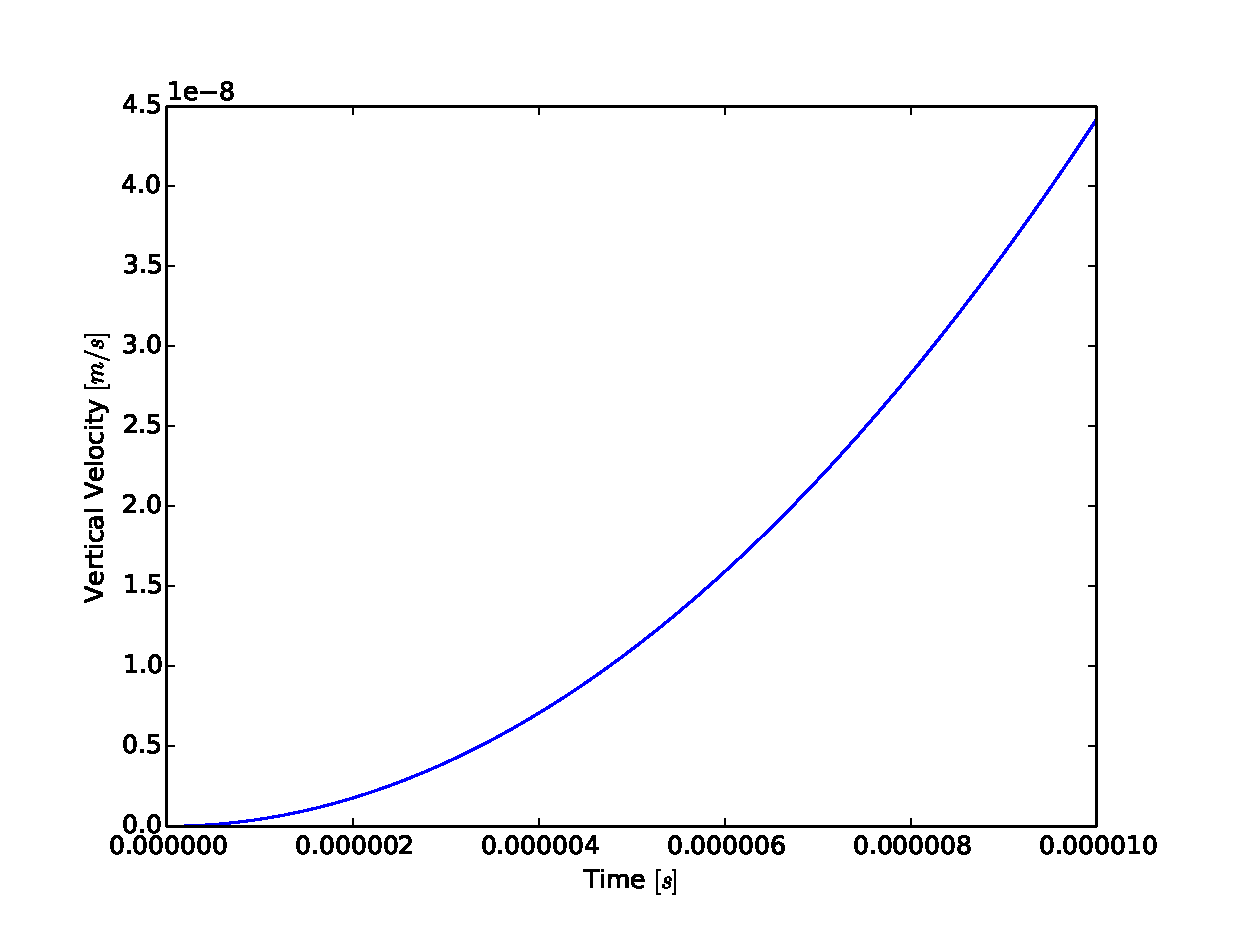
\includegraphics[width = 0.30\textwidth]{figures/7_0_12_vertical_vel}
      \caption{ The figures show a particle in the gyrating above the north pole, with a perpendicular velocity causing the gravitational and magnetic gradient force to balance. The figure to the shows the position, the center figure shows the positions as xyz coordinates and the figure to the right shows the vertical velocity.}
      \label{fig:no_perturbation}
    \end{figure}

  We first started the particle with a perpendicular velocity which had a balance between the magnetic gradient force and the gravitational force, so the vertical force the particle feels will be \(0\) and the particle will gyrate at the astarting point. This can be seen in \cref{fig:no_perturbation} although there is a very small increase in the vertical velocity which can be due to numerical errors.

  \begin{figure}
      \centering
      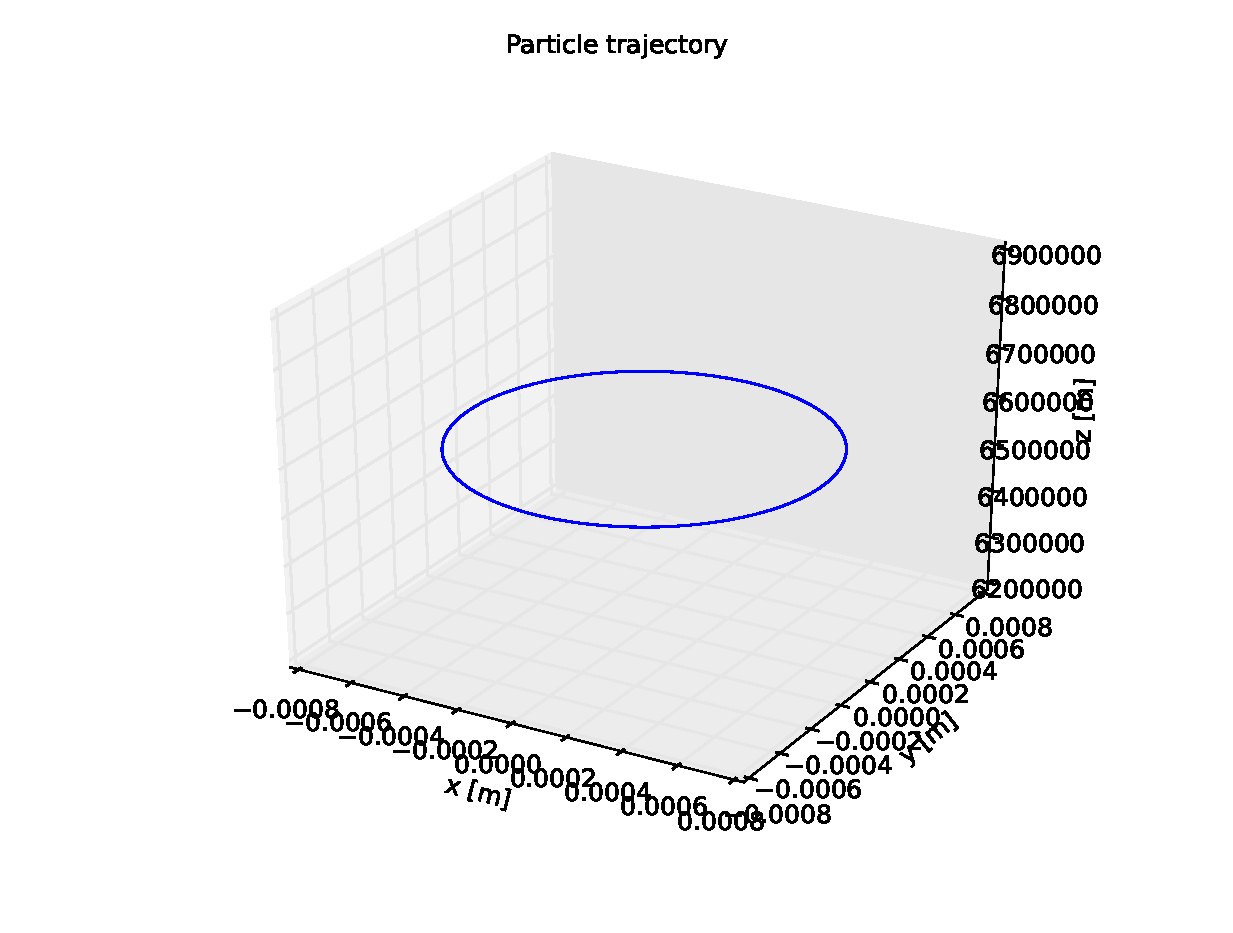
\includegraphics[width = 0.30\textwidth]{figures/7_-5_12_3Dplot}
      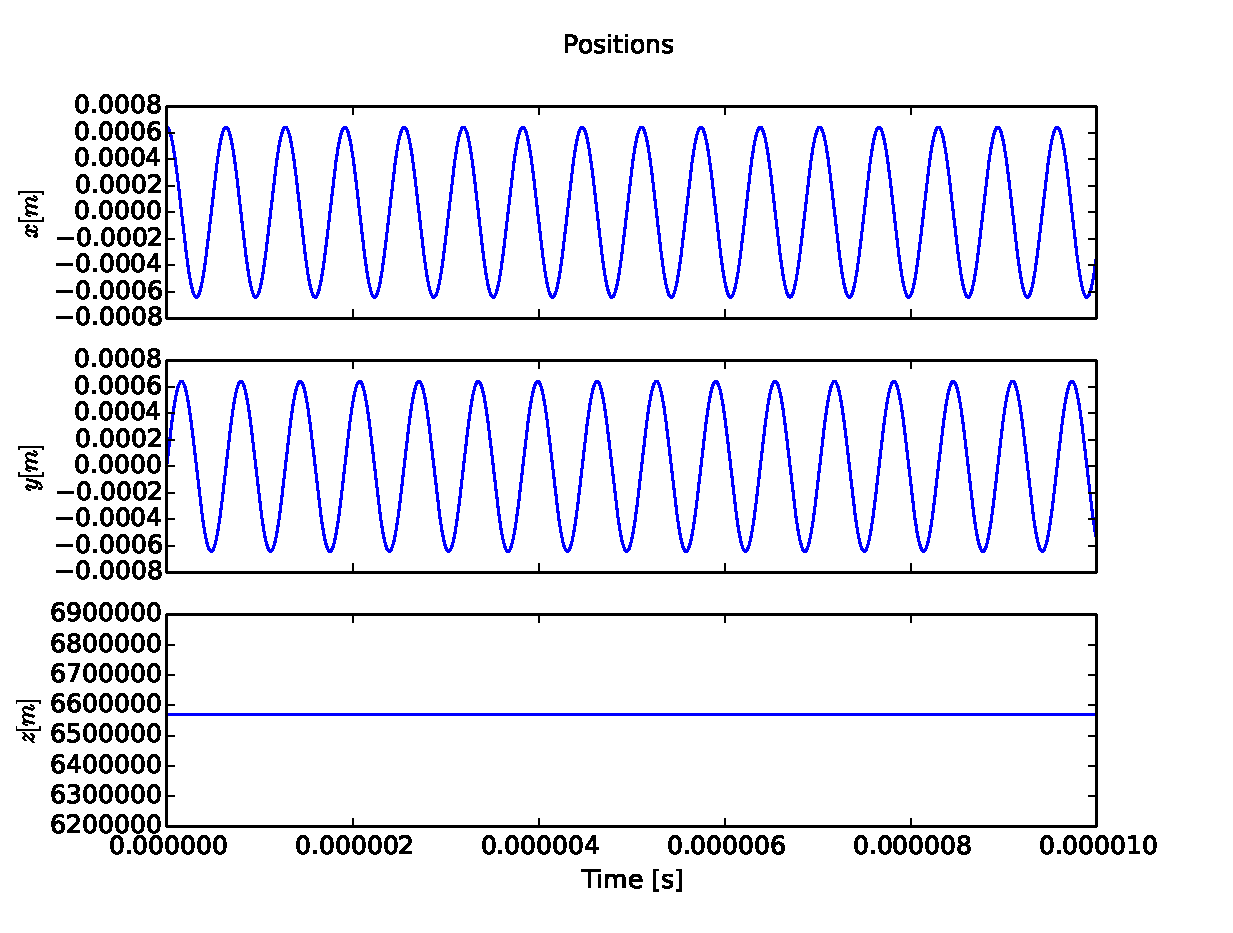
\includegraphics[width = 0.30\textwidth]{figures/7_-5_12_xyz}
      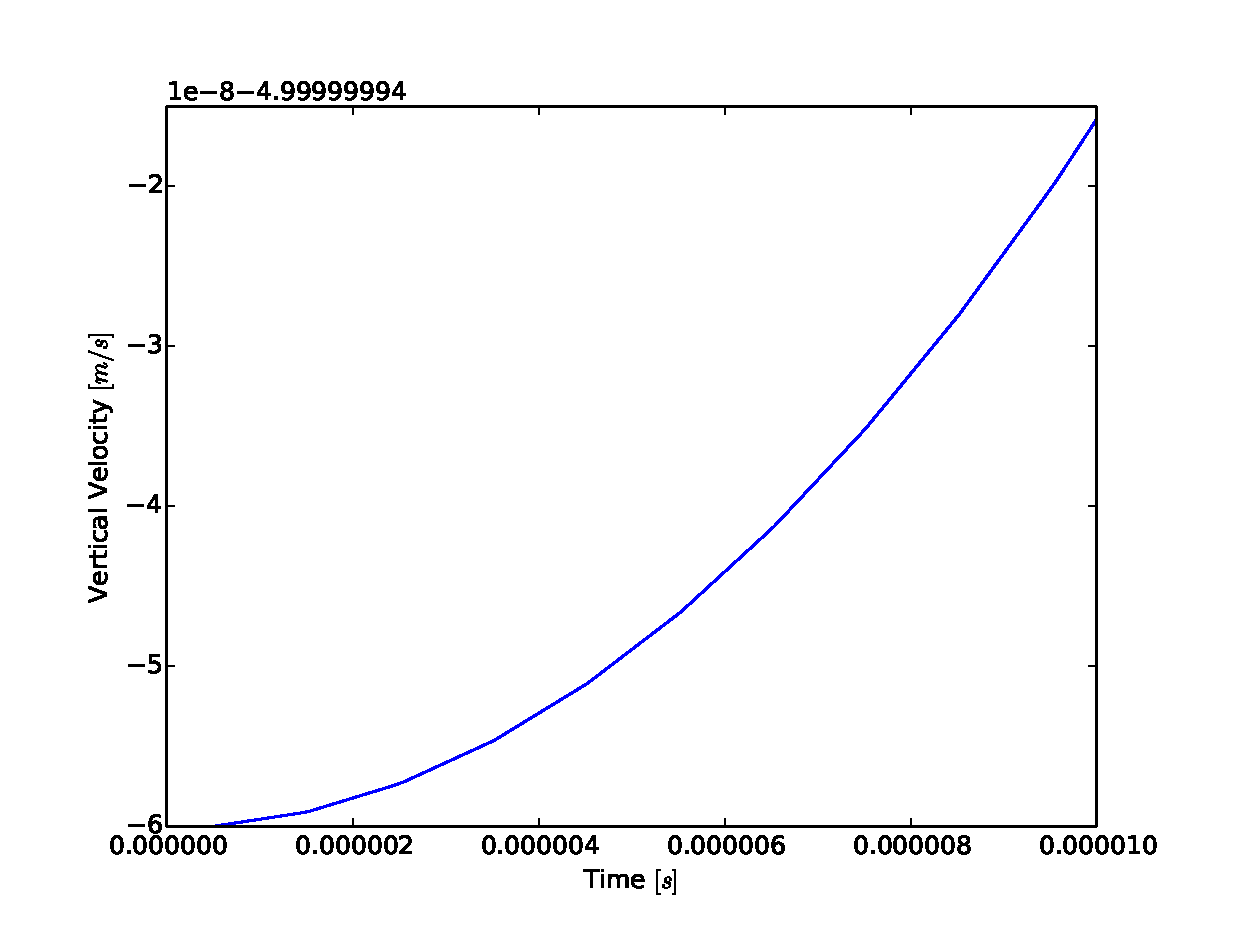
\includegraphics[width = 0.30\textwidth]{figures/7_-5_12_vertical_vel}
      \caption{ This particle started with a slight velocity toward the towards the earth of \(5 \si{\meter\per\second}\), this will cause the particle to move out of the height. The figure to the shows the position, the center figure shows the positions as xyz coordinates and the figure to the right shows the vertical velocity.}
      \label{fig:down_perturbation}
    \end{figure}

  \begin{figure}
      \centering
      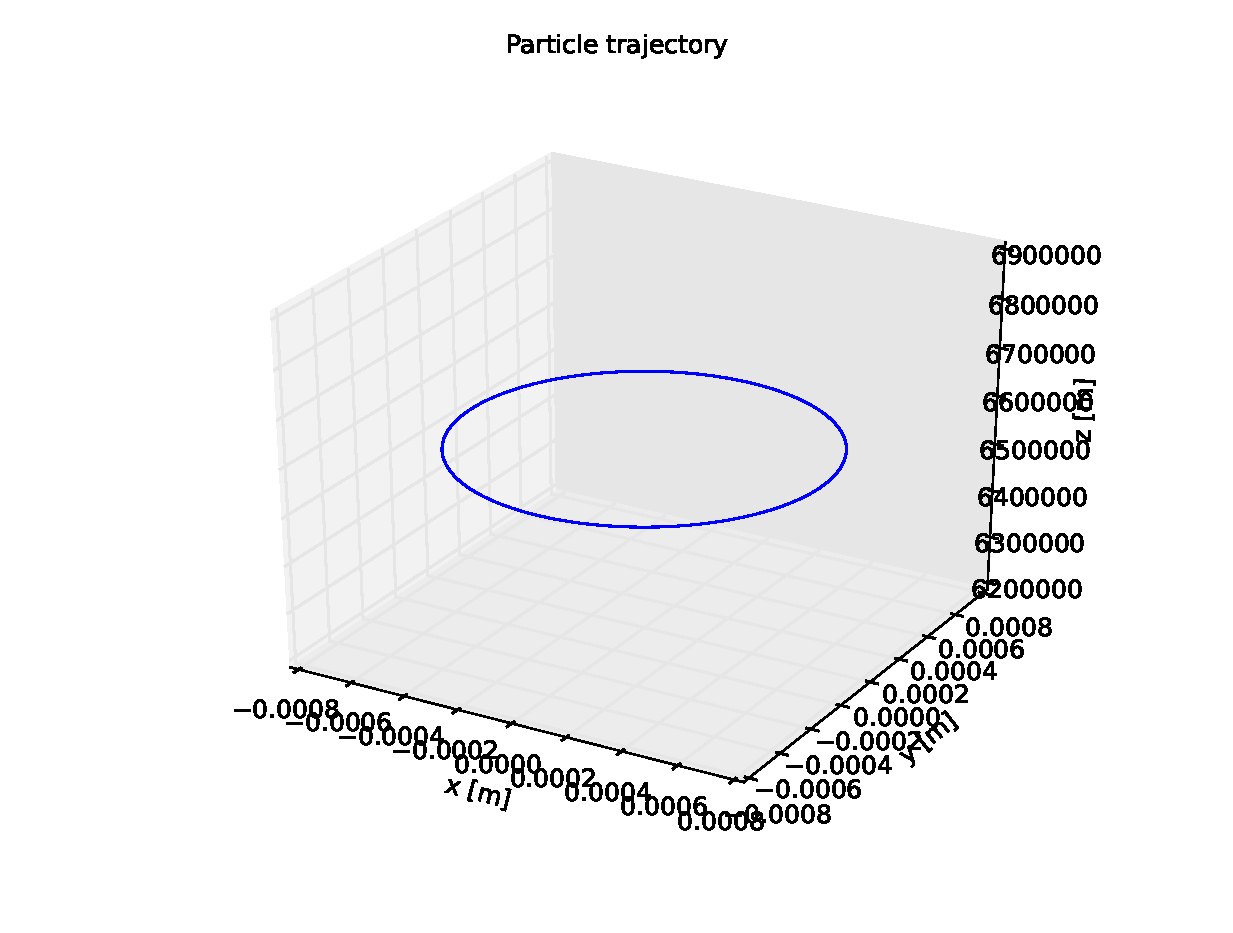
\includegraphics[width = 0.30\textwidth]{figures/7_5_12_3Dplot}
      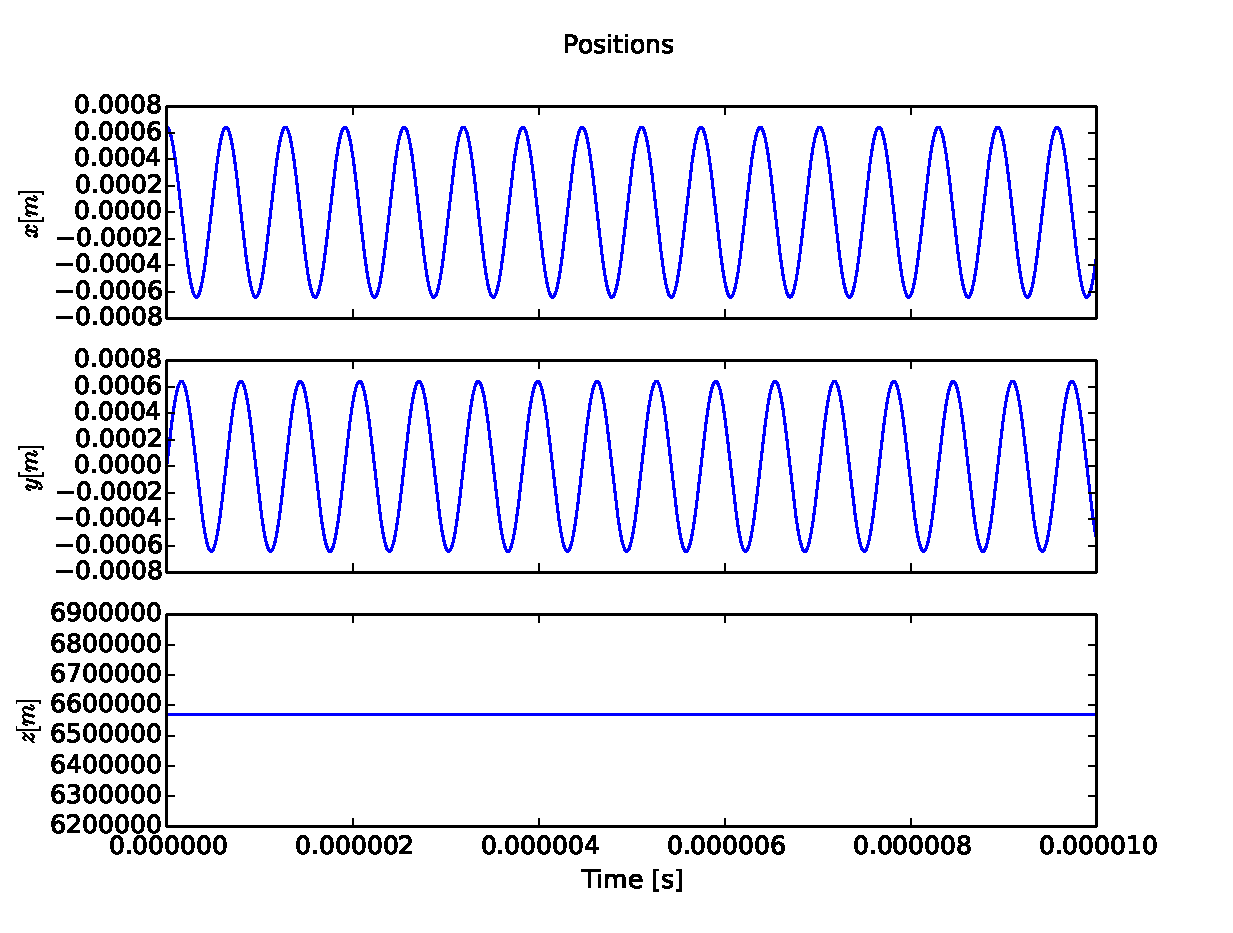
\includegraphics[width = 0.30\textwidth]{figures/7_5_12_xyz}
      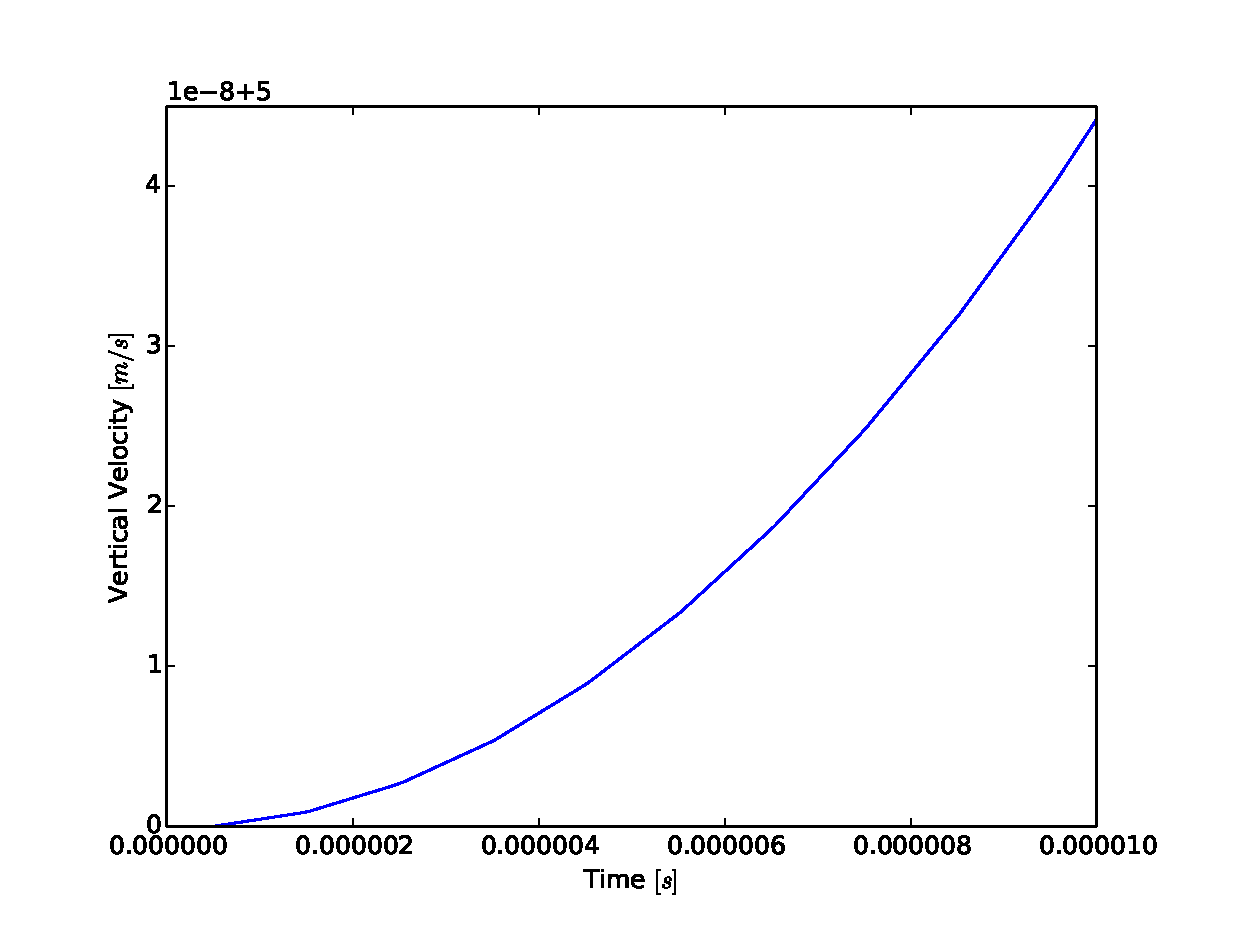
\includegraphics[width = 0.30\textwidth]{figures/7_5_12_vertical_vel}
      \caption{ This particle started with a slight velocity toward the towards the earth of \(5 \si{\meter\per\second}\), this will cause the particle to move out of the height. The figure to the shows the position, the center figure shows the positions as xyz coordinates and the figure to the right shows the vertical velocity.}
      \label{fig:up_perturbation}
   \end{figure}

  \cref{fig:down_perturbation,fig:up_perturbation} shows a particle with a slight downward velocity of \(5 \si{\meter\per\second}\), and the same upward velocity, which will cause the particle to move out the height at which the magnetic gradient force and the gravitational force will balance. As the particle begins to move downward gravitational force pulling it down will increase. In addition the gradient of the magnetic force will also increase. If the magnetic gradient force increases fastest when the particle moves down and the gravitational force increases fastest when it moves the particle will oscillate around the starting position. In any other relationship between the forces it will be in an unstable position at the start. Unfortunately the change in velocity is also registered in the first simulation when the particle had no initial perturbation so it is hard to conclude anything. (Will get back to this after I have implemented RK4)

\appendix

\section{Comments}
  \begin{itemize}
    \item I spoke to some students and everyone should be quite familiar with RK4 by the third year, so it should be done. Maybe it would be better to start RK4 in exercise 2, since it is a quite short exercise and then they won't have to write new code for exercise 3 which is quite abit more extensive.
    \item In the text it's written that the particle should be placed \(\frac{1}{2}\) a gyro radius to the side of magnetic pole. I assume we want to place the guiding center of the particle at the magnetic pole, which would need the particle to be placed \(1\) gyro radius to the side.
    \item On the exercise 1: It should probably have some part describing what they should do with the solved equations of motions, e.g. plot it and comment on the trajectory of the particle.
    \item Parenthesis around the magnetic field, equation \(5\).
    \item In equation \(6\) the equation of motion is listed as 
    \[m\pdv{\va{v}}{t} = q\va{v} \cross \va{B} - m \va{g}\]
    , and in equation \(7\) the gravity vector is listed as negative with respect to the direction.
    One of these should be positive so the gravitational force works the right direction (give a negative \(v_z\)).
    \item In the hint section the Earths mass has the wrong number, it should be to the power \(24\) instead of \(23\)
  \end{itemize}

\section{Code}
  \label{sec:code}
  \lstinputlisting{../source/stability.py}


\end{document}